\makeatletter
\setlength{\@fptop}{0pt}
\makeatother

%\subsection{Overall Architecture}
\begin{figure}[!t]
\centering
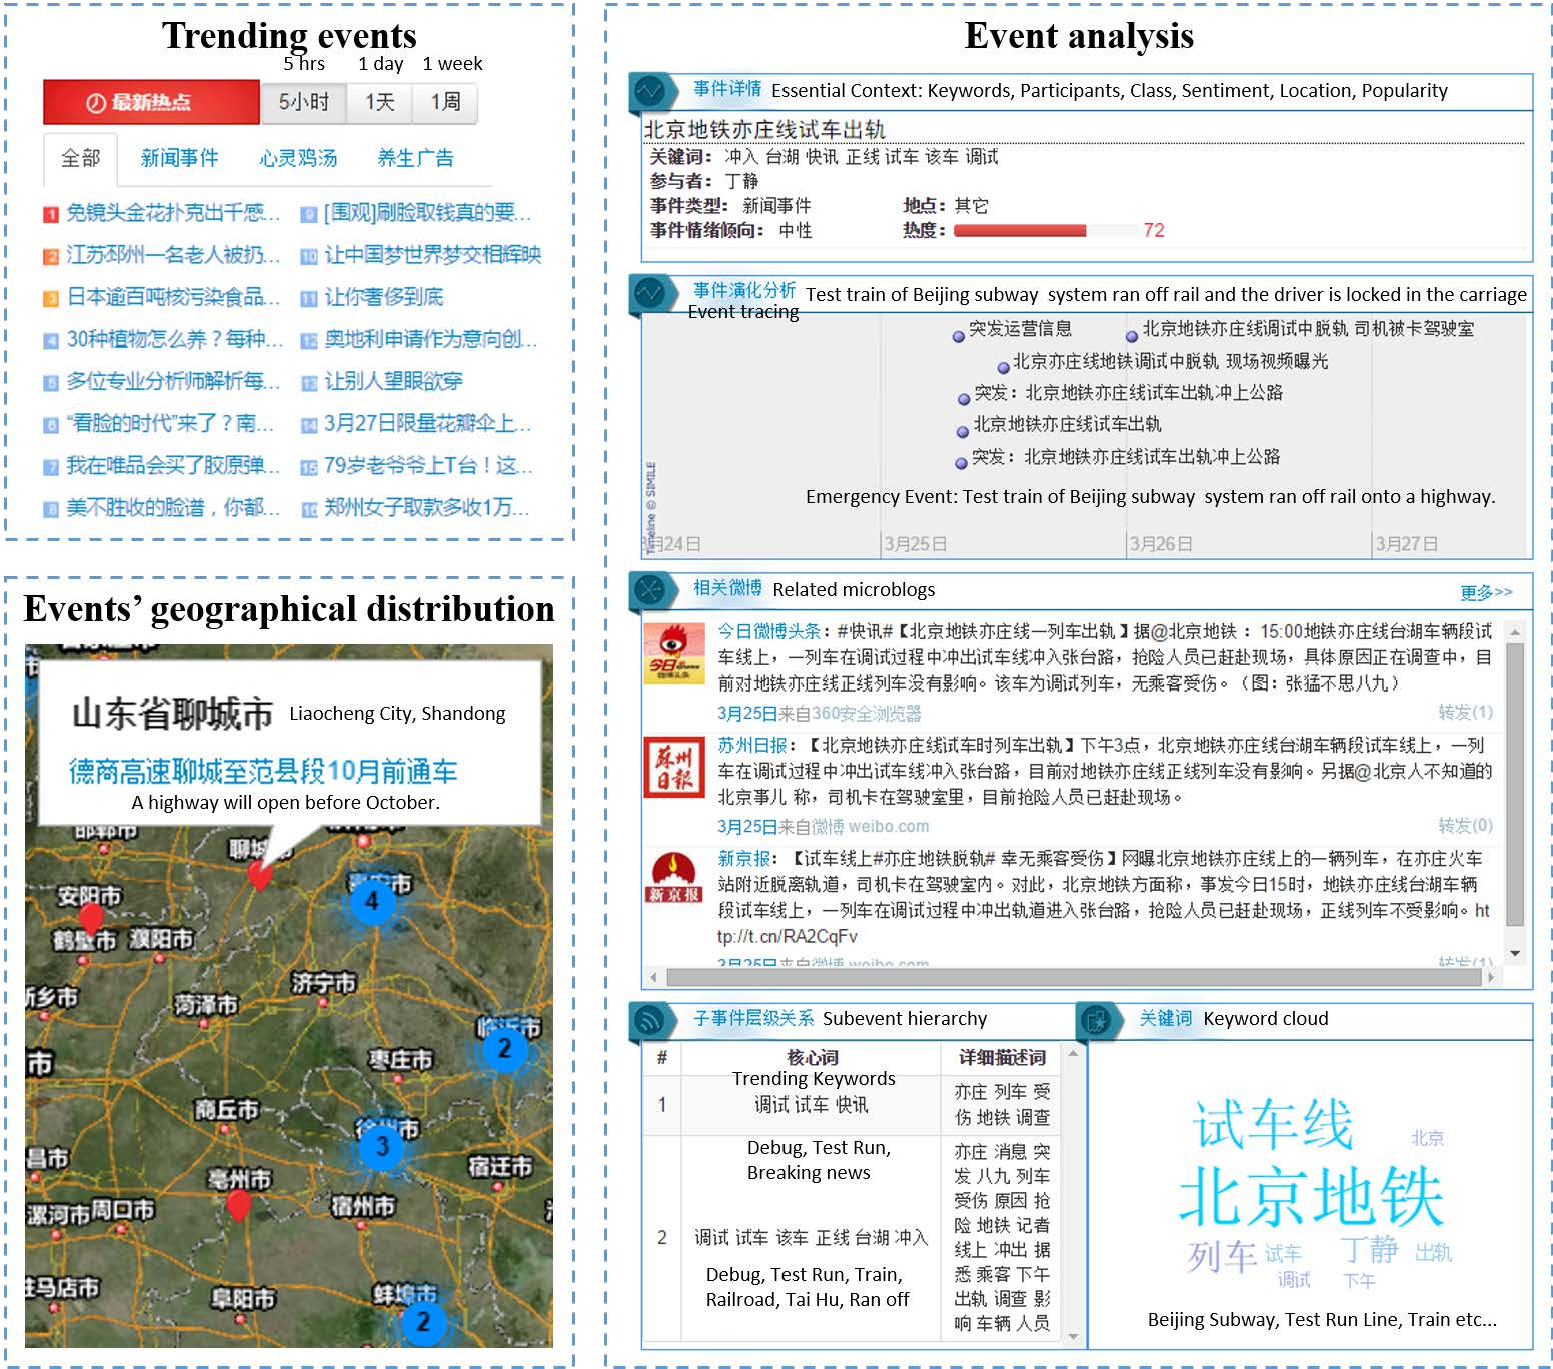
\includegraphics[width=3.3in, height=2.85in]{UI}
\caption{Features of Demonstration}
\label{fig:UI}
\end{figure}

%\subsection{User Interface}
\noindent\textbf{User Interface.}
We now introduce three function features to demonstrate emerging event monitoring as shown in Figure \ref{fig:UI}.

\emph{Trending Event Ranking:}
Events detected by \ring system are tracked based on the method mentioned in Section \ref{tracing}.
Events are ranked according to the volume of their related microblogs.
The ``hottest'' trending events in the past 5 hours, 1 day and 1 week are displayed on the front page of \ring system.
Our monitoring application could cover emerging events ahead of major news sites, \eg sina.com.cn or baidu.com.
Spam information has been effectively removed and missing events are majorly due to absence of data.
%There would be missing events

\emph{Event Analysis:}
Navigated from a search or trending event ranking, the event analysis page shows the detailed information of a detected event
which includes representative tweet as human-readable abstract, time of detection, keyword summarization, participants, event class as news or spam, location, sentiment bias and popularity.
The evolution the current event is displayed on a timeline interface, with related microblogs, sub-event hierarchy featuring trending keywords.
A word cloud of frequent keywords in related tweets is also displayed.

\emph{Geographical Distribution:}
The geographical distribution page shows a map with ballon markups indicating the number of events in the location.
Click on the ballons would display events in a specified location.
A search box allows users to query and navigate to the location more quickly.


\newcolumntype{C}{ >{\centering\arraybackslash} m{5.5cm} }
\newcolumntype{D}{ >{\centering\arraybackslash} m{1.8cm} }
\begin{table}
%\begin{minipage}[!t]{.5\textwidth}
%\raggedright
%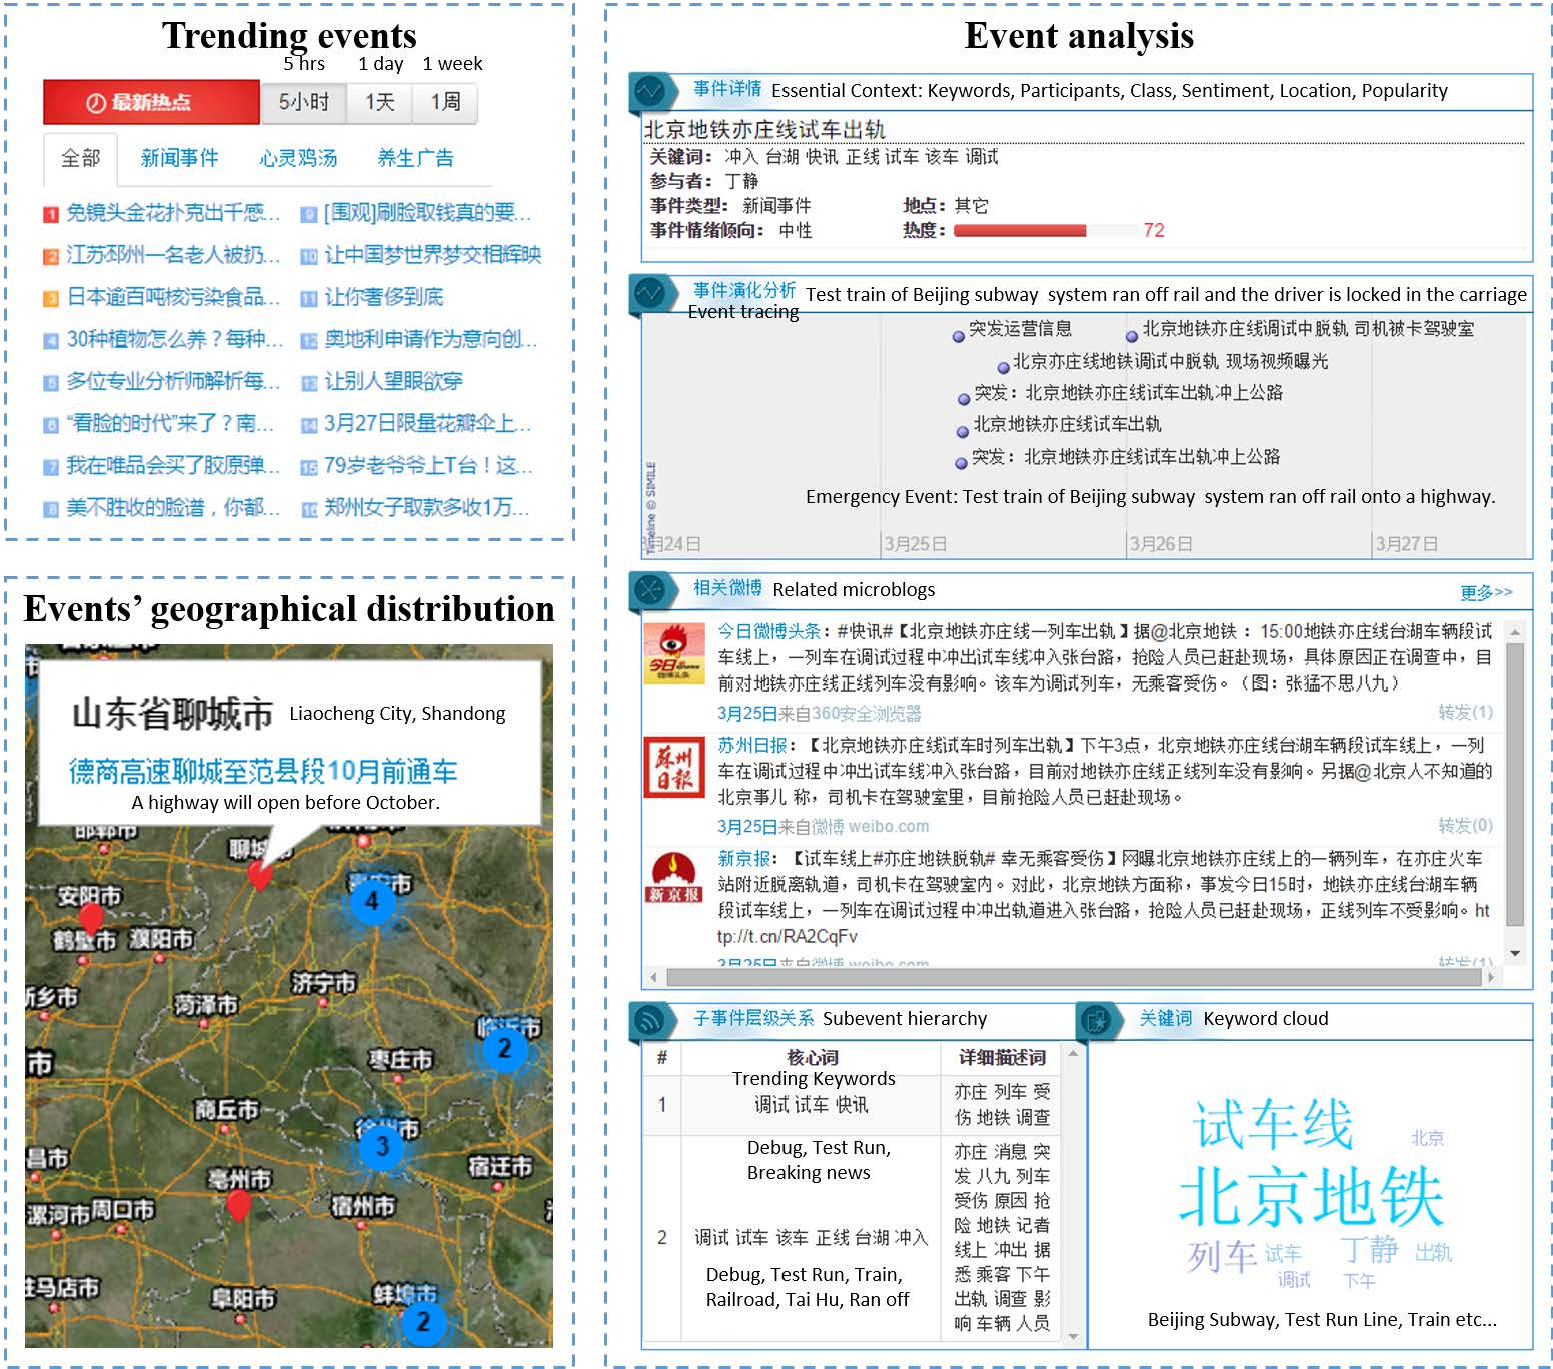
\includegraphics[width=3.3in, height=2.85in]{UI}
%\caption{Features for Demonstration}
%\label{fig:UI}
%\end{minipage}%\hfill
%\small
\raggedleft
\caption{A Case of Event Evolution Chain}
\begin{tabular}{|D|C|} \hline
\textbf{Time} & \textbf{Event description} \\ \hline
2014-12-01 18:40:00 & The suspect of Fudan poisoning case writes an apology letter to the victim's parents. $|$ The $2^{nd}$ trial will be held. \\ \hline
2014-12-08 08:10:00 & Fudan poisoning case's second trial will be held in 10am today, victim's parents will be in court. \\ \hline
2014-12-08 12:50:00 & LIVE: Defendant of Fudan poisoning case cries in court.\\ \hline
2015-01-08 07:40:00 & The court will pronounce judgement of the $2^{nd}$ trial today and victim's father hope to maintain the death penalty.\\ \hline
2015-01-08 10:30:00 & The court maintains the former death sentence on attempted murder in the second trail of Fudan poisoning case. \\ \hline
\end{tabular}
\label{fig:evolution}
\end{table}

\begin{table}
%\small
\raggedleft
\caption{A Case of Hierarchical Sub-Event}
\begin{tabular}{|D|C|}
\hline
\multirow{2}{1.8cm}{Poisoning Case, Fudan} & Apologize, Lin Senhao, Open a Court Session, Write \\ \cline{2-2}
                                           & Scheduled to, Shanghai \\ \hline
\end{tabular}
\label{fig:subevent}
\end{table}
